\documentclass{article}
\usepackage{listings}
\usepackage{graphicx}
\usepackage{float}
 
\floatstyle{ruled}
\newfloat{program}{thp}{lop}
\floatname{program}{Snippet}


\begin{document}

\title{Project Report - Limited Static Type Checking for JavaScript}
\author{Huascar A. Sanchez \and Tim Disney}

\maketitle

\lstset{showstringspaces=false}

\section{Introduction}
In the construction of software it is generally cheaper to 
catch programming errors earlier in the development cycle. One common method 
to catch errors is static type checking. This will
check the type consistency of the program before it is even
run. If the code has any type violations the type checker will 
find it and alert the programmer.

For example, in strongly typed languages like Java it is impossible 
to invoke a method which has not been defined for a class (unless reflection is used).
The compiler will immediately 
complain and prevent the program from compiling. However, in languages like 
JavaScript, this kind of error will not be discovered until runtime.

Adding static type checking to a dynamic language like JavaScript is a 
challenge, especially since objects can be modified at runtime. Given this challenge, 
we have implemented a static type checker, called JSCheck, for user-defined objects 
in JavaScript. The scope of JSCheck is limited to properties on an object's
prototype. In other words, we are completely ignoring type checking of the built in types
such as strings and numbers. The whole idea, as Lucas Cardelli said \cite{typesystems}, 
is to prevent the occurrence of errors during program execution. 

The rest of this paper is divided as follows. Section (\ref{sec:types}) gives an overview
of how user-defined types work in JavaScript, section (\ref{sec:implementation}) 
will discuss the design and implementation choices that were made through the development 
of JSCheck, related work will be discussed in (\ref{sec:related}), and future work
and conclusions in (\ref{sec:future}) and (\ref{sec:conclusion}).


\section{Types in JavaScript}
\label{sec:types}
User-defined types in JavaScript can be written in a variety of styles and forms. The form
that we considered in the scope of this project is object creation using 
constructor functions and prototype modification.

\begin{program}
\begin{verbatim}
function Dog(){
  // ..
}

Dog.prototype.getName = function(){
  //..
}

Dog.prototype.bark = function(){
  //..
}

var mydog = new Dog();
\end{verbatim}
\caption{Checking Types in JavaScript}
\label{fig:object}
\end{program}

For example, in code snippet (\ref{fig:object}) we define a {\tt Dog} type
which has two methods, {\tt getName} and {\tt bark} which are added to the {\tt Dog}
prototype. New ``instances'' of the {\tt Dog} type can be created with the {\tt new}
keyword.

There are other ways of creating objects including using object literal notation
and assigning methods directly to fields of an object but these techniques of 
object creation are not included in the scope JSCheck.

To enable JSCheck to check the usages of an object we add the comment type annotation
to the JavaScript language as seen in snippet \ref{fig:check}. In
this example the {\tt fido} parameter has been annotated with the {\tt Dog}
type in the {\tt //\#} comment. JSCheck will then check that all usages of
the {\tt fido} parameter conforms to the definition of the {\tt Dog} type.

\begin{program}
\begin{verbatim}
//# @type Dog fido
function useDog(fido) {
  fido.bark();
}

var mydog = new Dog();
useDog(mydog);
\end{verbatim}
\caption{Type Checking}
\label{fig:check}
\end{program}


\section{Implementation}
\label{sec:implementation}
JSCheck is implemented in Haskell. We were originally considering defining a 
subset of JavaScript to ease the burden of creating a parser for JavaScript. 
However we found a Haskell library called HJS \cite{hjsLibrary} 
which implements a full parser for JavaScript (ECMAScript 3rd edition plus 
some additions from JavaScript 1.5). We needed to make a few modifications to
HJS in order to pick up the type annotations but this greatly simplified much of
the effort in the implementation of JSCheck.

Figure \ref{fig:jscheckway} shows in general terms how JSCheck works. JSCheck takes 
in a JavaScript source file and runs
it through a modified version of the HJS parser. This produces an abstract syntax tree
which is then fed into a type extractor function which finds all the JavaScript 
object types that
have been defined. The output of this function is a list of types 
(type name and all associated fields)
which is given to a type checker function along with the original AST. The
checker function finds all functions that have been annotated with our special
type comments and checks all usages of typed parameters against the extracted types.
The final 
output will be a boolean representing if the code is well-typed or not. 

\begin{figure}[here]
  \begin{center}
    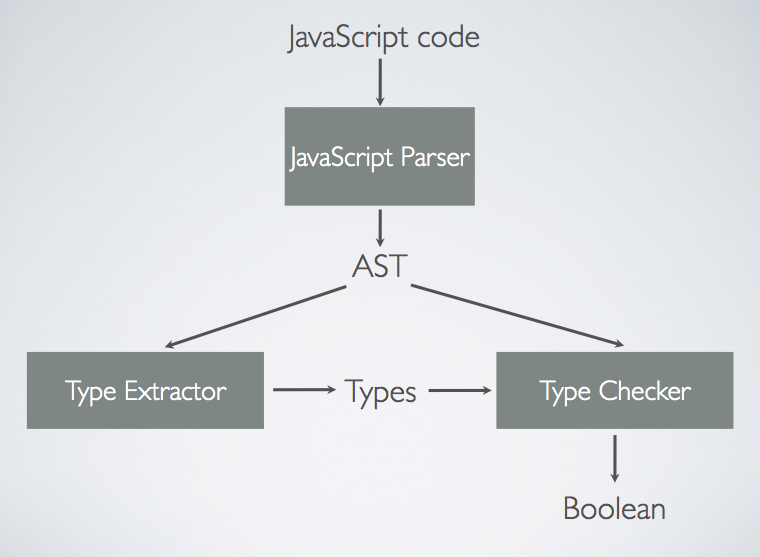
\includegraphics[scale=0.4]{blockdiagram.png}
  \end{center}
  \caption{Type Checking - the JSCheck way}
  \label{fig:jscheckway}
\end{figure}
\pagebreak

Because of the dynamic nature of JavaScript our implementation is both unsound 
and incomplete. It is unsound because methods could be added to the object at
runtime. So, even though the checker may find a usage of an unknown field, that field
might actually be defined. It is incomplete because fields could also be removed
from an object at runtime. The JavaScript program could be accessing non-existent 
fields even though the checker thought they were there.


\section{Related Work}
\label{sec:related}
We are not the first ones who have tried to implement static type checking for JavaScript.
There have been others who have done it before us. Some of them include:

\begin{description}
  \item[Tom Austin and Caitlin Sadowski] \hfill \\ 
  developed a structural type-checker for Javascript \cite{fwjsStruct}.
  \item[$JS_0$ team] \hfill \\ 
  developed a formalism for an object based language called JSO, which includes features of JavaScript 
  \cite{typeinferenceforjavascriptEcoop,typecheckingforjavascript}. 
  \item[DRuby team] \hfill \\ 
  developed Diamondback Ruby (DRuby), a tool that blends Ruby's dynamic type 
  system with a static typing discipline \cite{typecheckingruby}.
  \item[Google] developed the Closure compiler \cite{closureCompiler}.  
\end{description}

In some way, which remains obscure, we all shared the same drive for making type 
checking possible in a dynamic language. We chose JavaScript for many reasons. 
However, the most important one, for us, was that JavaScript is the most used 
language in the World Wide Web and providing this type checking capability would
be appreciated by many. 

Our implementation is both unsound and incomplete. One thing that sets our 
implementation apart for previous work is that our checker works (in a limited 
fashion) for full JavaScript.

One thing that sets our 
implementation apart for previous work is that our checker works (in a limited fashion) for
full JavaScript.

\section{Future Work}
\label{sec:future}
There are several areas in our static type checker that could be expanded. One of
them, as indicated above, is the type checking output. Future will be focused on 
providing a more descriptive type checking output. Another extension could be to
provide type consistency checks for other elements of the language, like strings
and numbers.

%TODO: talk about other forms of object creation


\section{Conclusion}
\label{sec:conclusion}
We have developed a static type checker for prototype based objects in JavaScript
called JSCheck. By using this checker any developer will be able to catch any 
type errors before running their programs. The only thing the developer needs to
do is to explicitly type annotate a function(s). The rest is done by JSCheck. 

The idea of implementing a type checker strongly motivated us. It is hard for us 
describe the feeling of accomplishment after completing our implementation. Now,
for sure, we have a better understanding of what static type checking is all about. 

Full source can be found at {\tt http://github.com/disnet/jscheck}.

\bibliographystyle{abbrv}
\bibliography{report}

\end{document}


